\documentclass[12pt,a4paper]{article}

% --- Настройка языка и шрифтов для LuaLaTeX ---
\usepackage{fontspec}
\defaultfontfeatures{Ligatures=TeX,Scale=MatchLowercase}

\setmainfont{Alice-Regular}[
    Path=font/,
    Extension=.ttf,
    BoldFont = Alice-Regular,
    ItalicFont = Alice-Regular,
    BoldItalicFont = Alice-Regular,
    BoldFeatures = {FakeBold=1.6},
    ItalicFeatures = {FakeSlant=0.2},
    BoldItalicFeatures = {FakeBold=1.6,FakeSlant=0.2}
]

\newfontfamily\cyrillicfont{Alice-Regular}[
    Path=font/,
    Extension=.ttf,
    BoldFont = Alice-Regular,
    ItalicFont = Alice-Regular,
    BoldItalicFont = Alice-Regular,
    BoldFeatures = {FakeBold=1.6},
    ItalicFeatures = {FakeSlant=0.2},
    BoldItalicFeatures = {FakeBold=1.6,FakeSlant=0.2}
]

\usepackage{polyglossia}
\setmainlanguage{russian}
\setsansfont{TeX Gyre Heros}
\setmonofont{TeX Gyre Cursor}

\usepackage{graphicx}        					          % Графика
\usepackage[protrusion=false]{microtype}       	% Микротипографика
\usepackage{amsmath, amsfonts, amssymb, amsthm}	% Математика
\usepackage{braket} 							              % Braket нотация для квантовой механики
\usepackage{unicode-math} 						          % Современный пакет для математики в LuaLaTeX
\usepackage{longtable}       					          % Таблицы с разрывом страниц
\usepackage{tikz}           					          % Рисование
\usepackage[europeanresistors]{circuitikz}		  % Рисование электрических схем в европейском стиле
\usepackage{listings}							              % Для отображения кода
\usepackage{tabularx}       					          % Для таблиц во всю ширину
\usepackage{array}		  						            % Для расширенных возможностей таблиц
\usepackage{float}          					          % Для точного позиционирования фигур
\usepackage{pgfplots}                           % Для построения графиков
\usepackage{caption}                            % Для настройки подписей к рисункам и таблицам
\usepackage{xfp}                                % Для вычислений в LaTeX
\pgfplotsset{compat=1.18}
\usepackage[a4paper,left=20mm,right=20mm,top=20mm,bottom=20mm]{geometry}

\usetikzlibrary{arrows.meta}

% --- Колонтитулы ---
\usepackage{fancyhdr}
\pagestyle{fancy}
\fancyhf{}

\renewcommand{\headrulewidth}{0.4pt}
\renewcommand{\footrulewidth}{0.4pt}
\renewcommand\lstlistingname{Исходный код}

\lstdefinestyle{main}{
	backgroundcolor=\color{gray!8},   
	commentstyle=\color{green!50!black},
	keywordstyle=\color{blue!80!black},
	numberstyle=\small\color{darkgray},
	stringstyle=\rmfamily\color{orange!90!black},
	basicstyle=\ttfamily\small,
	breakatwhitespace=false,         
	breaklines=true,                   
	keepspaces=true,                 
	numbers=left,                    
	numbersep=8pt,                  
	showspaces=false,                
	showstringspaces=false,
	showtabs=false,                  
	tabsize=4
}	

\lstset{style=main}

\newcolumntype{C}{>{\centering\arraybackslash}X}
\renewcommand{\arraystretch}{1.25}

% =========================================================
%         СЛУЖЕБНЫЕ КОМАНДЫ ДЛЯ ВЫЧИСЛЕНИЙ
% =========================================================
\newcommand{\CalcTwo}  [1]{\fpeval{round((#1),2)}}
\newcommand{\CalcThree}[1]{\fpeval{round((#1),3)}}
\newcommand{\CalcFour} [1]{\fpeval{round((#1),4)}}
\newcommand{\CalcFive} [1]{\fpeval{round((#1),5)}}

% ---------------------------------------------------------
% ОБЩИЕ ДАННЫЕ
% ---------------------------------------------------------
\def\VariantN{1}          					         % Номер варианта
\def\StudentName{Андреев Иван Алексеевич}  	 % ФИО студента
\def\TeacherName{Устинов Юрий Александрович} % ФИО преподавателя
\def\LabNumber{1}							               % Номер лабораторной работы
\def\Discipline{Дисциплина}				           % Название дисциплины
\def\LabTitle{Название лабораторной работы}	 % Название лабораторной работы

\title{
	МИНОБРНАУКИ РОССИИ

	федеральное государственное автономное образовательное учреждение

	высшего образования

	«Национальный исследовательский университет
	«Московский институт электронной техники»
	\vspace{2em}
}
\author{
}
\date{}

\begin{document}

\maketitle
\thispagestyle{fancy}

\begin{center}
\Large Отчёт по Лабораторной работе $\LabNumber$\\
по дисциплине «\Discipline»\\
«\LabTitle»
\end{center}

\begin{center}
\Large Вариант \VariantN
\end{center}

\vspace{12em}

\begin{table}[h]
\noindent
\begin{tabular*}{\textwidth}{@{\extracolsep{\fill}} p{0.48\textwidth} p{0.52\textwidth}}
Студент, группа & \StudentName, ЭН-$25$ \\
[0.5em] Руководитель & \TeacherName
\end{tabular*}
\end{table}

\cfoot{Москва 2026}

\pagebreak

\fancyhead[L]{\LabTitle} 
\fancyhead[R]{\Discipline}
\fancyfoot[C]{\thepage}

% Пример правильной вставки кода на языке Matlab, начиная с 12 строки файла free_movement.m
\begin{lstlisting}[language=Matlab, firstnumber=12, 
	title={\textbf{free\_movement.m}}]
m = 9.1e-31;                % mass of electron (kg)
h = 1.05e-34;               % Plank's constant (J*s)
E0 = 20;                    % energy of electron (eV)
v0 = sqrt(2*E0*1.6e-19/m);  % velocity of electron (m/s)
d0 = 1;                     % half-width of wave packet (A, Angstroem)
x0 = 10.0;                  % center of wave packet (A, Angstroem)

%-------------------------------------------------------------
% TINE AND SPACE PARAMETERS

% time points, (fs, femtosecond)
t0 = 0;
t1 = 0.1;       
t2 = 0.2;
t3 = 0.3;
t4 = 0.4;

% begin and end of line segment of axis 'x'
xBegin = 5;
xEnd = 35;
\end{lstlisting}

% пример оформления формулы или вывода для последующего использования в расчётах
\begin{equation}
	E_0 = \frac{p_0^2}{2m_{e^-}} \Longrightarrow p_0 = \sqrt{2m_{e^-}E_0}
\end{equation}

% пример оформления обычного расчёта 
\begin{equation*}
  \begin{aligned}
    U_{R_1} &= I_1 \cdot R_1 = 2.02 \cdot 1 = 2.02\,\text{В} \\
    U_{L_1} &= I_1 \cdot X_{L_1} = 2.02 \cdot j = 2.02j\,\text{В} \\
    U_{C_2} &= I_2 \cdot X_{C_2} = (-1.01 + 1.01j) \cdot (-5j) = 5.05 + 5.05j\,\text{В} \\
    U_{R_3} &= I_3 \cdot R_3 = (3.03 - 1.01j) \cdot 1 = 3.03 - 1.01j\,\text{В} \\
    U_{L_3} &= I_3 \cdot X_{L_3} = (3.03 - 1.01j) \cdot 2j = 2.02 + 6.06j\,\text{В} \\
  \end{aligned}
\end{equation*}

% пример векторно-топографической диаграммы для контуров
\begin{figure}[H]
  \centering
    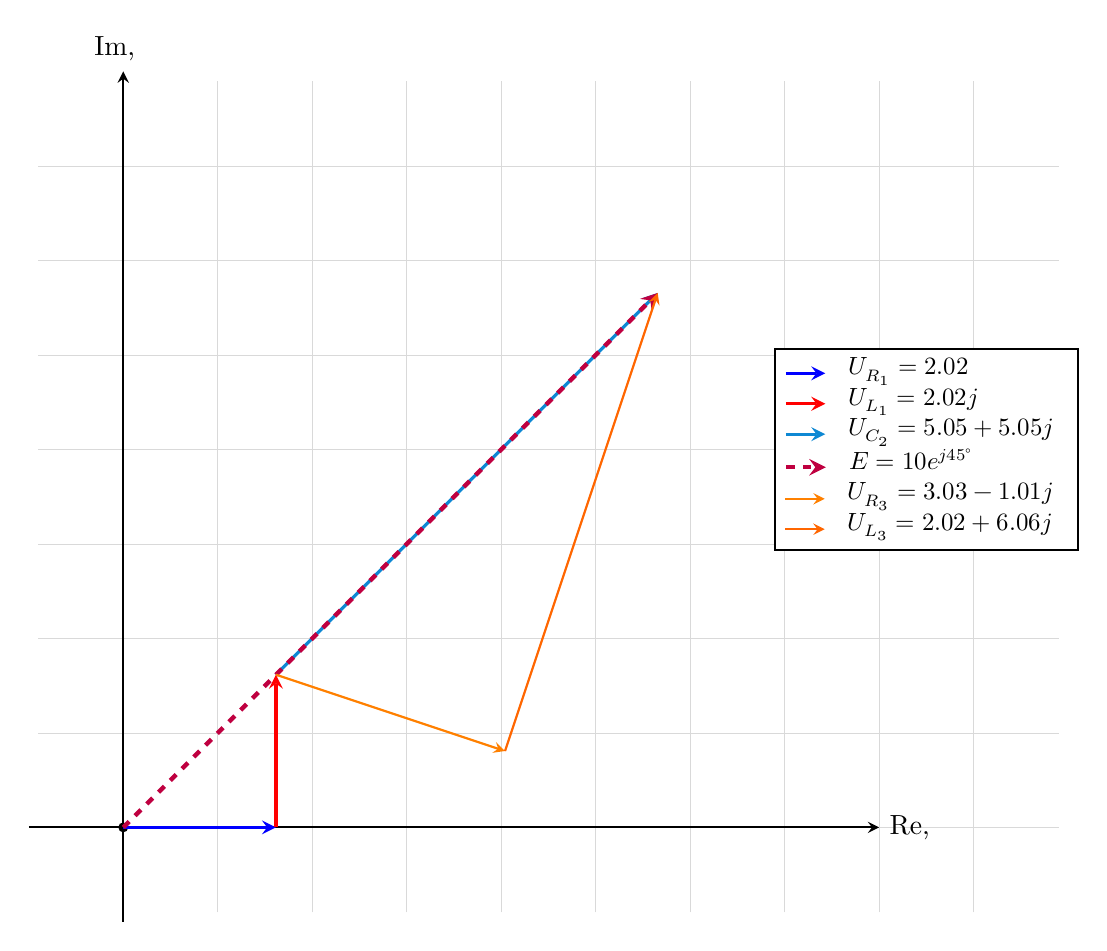
\begin{tikzpicture}[scale=1.2, >=stealth]
      % Масштабный коэффициент для удобства отображения
      \def\scale{0.8}
      
      % Сетка
      \draw[gray!30, very thin] (-0.9,-0.9) grid[step=1] (9.9,7.9);
      
      % Оси координат
      \draw[->, thick] (-1, 0) -- (8, 0) node[right] {Re, В};
      \draw[->, thick] (0, -1) -- (0, 8) node[above] {Im, В};
      
      % Точка начала (общая точка)
      \fill[black] (0,0) circle (1.5pt);
      
      % Вектор U_{R_1} = 2.02 В (по оси Re)
      \draw[->, very thick, blue] (0,0) -- (2.02*\scale,0);
      \fill[blue] (2.02*\scale,0);
      
      % Вектор U_{L_1} = 2.02j В (по оси Im)
      \draw[->, very thick, red] (2.02*\scale,0) -- (2.02*\scale,2.02*\scale);
      \fill[red] (2.02*\scale,2.02*\scale);
      
      % Вектор U_{C_2} = 5.05 + 5.05j В
      \draw[->, very thick, cyan!70!blue] (2.02*\scale,2.02*\scale) -- (2.02*\scale+5.05*\scale,2.02*\scale+5.05*\scale);
      \fill[cyan!70!blue] (2.02*\scale+5.05*\scale,2.02*\scale+5.05*\scale);
      
      % Вектор источника E (от начала до конца - пунктиром)
      \draw[->, ultra thick, purple, dashed] (0,0) -- (2.02*\scale+5.05*\scale,2.02*\scale+5.05*\scale);
      
      % Альтернативный путь через R_3 и L_3
      % U_{R_3} = 3.03 - 1.01j
      \draw[->, thick, orange] (2.02*\scale,2.02*\scale) -- (2.02*\scale+3.03*\scale,2.02*\scale-1.01*\scale);
      \fill[orange] (2.02*\scale+3.03*\scale,2.02*\scale-1.01*\scale);
      
      % U_{L_3} = 2.02 + 6.06j
      \draw[->, thick, orange!80!red] (2.02*\scale+3.03*\scale,2.02*\scale-1.01*\scale) -- 
      (2.02*\scale+5.05*\scale,2.02*\scale+5.05*\scale);
      
      % Легенда
      \node[draw, thick, fill=white, align=left, font=\small] at (8.5, 4) {
        \tikz \draw[->, very thick, blue] (0,0) -- (0.5,0); \, $U_{R_1}=2.02$ В \\
        \tikz \draw[->, very thick, red] (0,0) -- (0.5,0); \, $U_{L_1}=2.02j$ В \\
        \tikz \draw[->, very thick, cyan!70!blue] (0,0) -- (0.5,0); \, $U_{C_2}=5.05+5.05j$ В \\
        \tikz \draw[->, ultra thick, purple, dashed] (0,0) -- (0.5,0); \, $E=10e^{j45^\circ}$ В \\
        \tikz \draw[->, thick, orange] (0,0) -- (0.5,0); \, $U_{R_3}=3.03-1.01j$ В \\
        \tikz \draw[->, thick, orange!80!red] (0,0) -- (0.5,0); \, $U_{L_3}=2.02+6.06j$ В
        };
        
      \end{tikzpicture}
      \caption{Векторно-топографическая диаграмма для контура с элементами $R_1$, $L_1$, $C_2$, $R_3$ и $L_3$.}
      \label{fig:vector_diagram}
  \end{figure}
    
    % пример оформления таблицы
\begin{center}
  \begin{table}[H]
    \noindent
    \begin{tabularx}{\textwidth}{|C|C|C|C|C|C|C|}
		\hline
		$p_0$, \text{кг·Å/фс} & $\sigma_p$, \text{кг·Å/фс} & $P\{-\infty < p \leq p_0 - \sigma_p\}$ & $P\{p_0 - \sigma_p \leq p \leq p_0 + \sigma_p\}$ & $P\{p_0 + \sigma_p \leq p < +\infty\}$ \\
		\hline
		$24.16 \times 10^{-30}$ & $7.43 \times 10^{-30}$ & $0.158645 \pm 0.00001$ & $0.68271 \pm 0.00002$ & $0.158645 \pm 0.00001$ \\
		\hline
		\end{tabularx}
		\caption{Результаты расчёта параметров распределения вероятности по импульсам для $E_0 = 20$ эВ и $d_0 = 1$ Å.}
		\label{tab:lab2qmTask5part1}
	\end{table}
\end{center}

\end{document}